
\section{Das Relativitätsprinzip 
\label{relativ:section:relativistik}}
\rhead{Das Relativitätsprinzip}

Um relativistische Mechanik verstehen zu können,
muss natürlich zuerst auf das Relativitätsprinzip eingegangen werden.
Dabei gibt es zwei wesentliche Unterschiede zur klassischen Mechanik.

Der erste wichtige Unterschied ist, dass die Zeit unter relativistischer Betrachtung keine absolute Grösse ist.
Geschehenes kann also nicht einfach anhand eines starren Zeitstrahls erklärt werden, sondern die Zeit ist abhängig vom Betrachter.
Man geht über vom dreidimensionalen Raum in die vierdimensionale Raumzeit, in welcher die Welt relativistisch beschrieben wird.
Punkte in dieser Raumzeit werden als \emph{Ereignisse} oder \emph{Weltpunkte} bezeichnet.

Der zweite Unterschied ist,
dass die Geschwindigkeit der Wirkungsausbreitung begrenzt ist,
und zwar durch die Lichtgeschwindigkeit
\(c=\num{299792458}\unit[per-mode = fraction]{\metre\per\second}\).
Diese ist zwar auch in der klassischen Mechanik eine Konstante,
jedoch ist die Geschwindigkeit der Wirkungsausbreitung dort unbegrenzt.
Ein einfaches Beispiel, um dies zu veranschaulichen,
ist die Betrachtung von starren Körpern in der klassischen Mechanik.
Wird ein starrer Körper beispielsweise an einem Punkt angestossen,
so muss sich, gemäss Definition eines starren Körpers,
jeder Teil dieses Körpers augenblicklich und zeitgleich in Bewegung setzen.
Dies bedeutet also, dass sich die Wirkung (Anstossen des Körpers)
vom Punkt aus, in dem dieser angestossen wurde,
mit unendlicher Geschwindigkeit in alle Teile des Körpers ausbreitet.
Unter relativistischer Betrachtung ist dies also nicht möglich,
und es kann somit auch keine starren Körper geben.


\subsection{Der Abstand 
\label{relativ:section:abstand}}

Ebenfalls muss der Begriff des Abstands für die relativistische Mechanik umformuliert werden.
In der klassischen Mechanik ist der euklidische Abstand
\begin{equation}
    ds=\sqrt{dx^2 + dy^2 + dz^2}
    \label{relativ:eqn:abstand-klass}
\end{equation}
in den drei Raumkoordinaten \(x, y, z\)
für alle Bezugssysteme identisch.

Analog dazu gibt es in der relativistischen Mechanik den erweiterten Abstand
\begin{equation}
    ds = \sqrt{c^2dt^2 - dx^2 - dy^2 - dz^2}
    \label{relativ:eqn:abstand-relativ}
\end{equation}
in den Koordinaten \(ct, x, y, z\) der Raumzeit.
Dieser ist ebenfalls für verschiedene Bezugssysteme identisch.
Ausgehend von der Invarianz des Abstandes lassen sich
viele Gesetze der relativistischen Mechanik herleiten.


\subsection{Die Eigenzeit 
\label{relativ:section:eigenzeit}}

Angenommen, wir beobachten eine Uhr,
welche sich in unserem Koordinatensystem um die Strecke
\(\sqrt{dx^2 + dy^2 + dz^2}\)
bewegt.
Im Koordinatensystem der Uhr gilt
\(dx' = dy' = dz' = 0\).
Gemäss der Invarianz des Abstands gilt somit
\begin{equation*}
    \underbrace{ds^2 = c^2 dt^2 - dx^2 - dy^2 - dz^2}_{\text{Unser Koordinatensystem}}
        = \underbrace{ds'^2 = c^2 dt'^2}_{\text{Koordinatensystem der Uhr}} .
\end{equation*}
Wird dieser Ausdruck nach dem Differential der Zeit im System der Uhr aufgelöst,
so folgt
\begin{equation}
    dt' = \frac{ds}{c} = \frac{ds'}{c}
    = dt \sqrt{1 - \frac{dx^2+dy^2+dz^2}{c^2 dt^2}}
    = dt \sqrt{1 - \frac{v^2}{c^2}},
    \label{relativ:eqn:differential-eigenzeit}
\end{equation}
mit der Geschwindigkeit \(v\) der Uhr.
Dieses Zeitdifferential kann nun zur Zeitdifferenz
\begin{equation}
    t_2' - t_1' = \int_{t_1}^{t_2} dt \sqrt{1 - \frac{v^2}{c^2}}
    \label{relativ:eqn:eigenzeit}
\end{equation}
integriert werden.
Das ist nun die Zeit, die von der bewegten Uhr gemessen wird.
Eine solche Zeit, welche von einer Uhr,
die sich mit einem Gegenstand mitbewegt, gemessen wird,
nennt man \emph{Eigenzeit}.
Durch den Ausdruck unter der Wurzel wird klar,
dass die Zeitdifferenz \(t_2'- t_1'\) kleiner ist
als \(t_2 - t_1\) im Referenzsystem.
Daher kommt auch der Ausdruck
``bewegte Uhren gehen langsamer''.


\subsection{Koordinatentransformationen 
\label{relativ:section:koordtrafo}}

Koordinatentransformationen werden benutzt,
um Koordinaten aus einem Bezugssystem in diejenigen eines anderen Bezugssystems umzurechnen.
In der Physik dienen sie beispielsweise dazu,
ein System oder einen Vorgang aus einer anderen Perspektive bzw.
von einem anderen Referenzpunkt aus zu beschreiben.

\subsubsection{Galilei-Transformation 
\label{relativ:section:galilei-trafo}}

In der klassischen Mechanik gibt es die folgenden,
intuitiven Transformationen, um zwischen verschiedenen Bezugssystemen
zu vergleichen:
\[
\begin{aligned}
    &\text{Translation in der Zeit: } && t \rightarrow t + b \\
    &\text{Translation im Raum: } && \vec{r} \rightarrow \vec{r} + \vec{a} \\
    &\text{Orthogonale Drehung: } && \vec{r} \rightarrow A \vec{r} \\
    &\text{Transformation auf ein Bezugssystem mit Relativgeschwindigkeit: } && \vec{r} \rightarrow \vec{r} + \vec{v} \cdot t .
\end{aligned}
\]
Eine Kombination aus diesen Transformationen wird als Galilei-Transformation bezeichnet.
Ein einfaches Beispiel dafür ist in Abbildung~\ref{relativ:fig:galilei-trafo} zu finden.
\begin{figure}
    \centering
    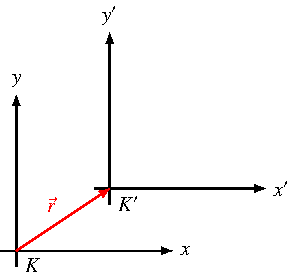
\includegraphics{papers/relativ/tikz/galilei_trafo.pdf}
    \caption{Darstellung einer einfachen Galilei-Transformation in \(\mathbb{R}^2\)
    vom Koordinatensystem \(K\) zum System \(K'\).
    Sie besteht lediglich aus einer Translation um den Vektor \(\vec{r}\).
    \label{relativ:fig:galilei-trafo}}
\end{figure}
Die Galilei-Transformation bildet die Grundlage für die Methoden der klassischen Mechanik,
wie beispielsweise die Addition von Kräftevektoren.

\subsubsection{Lorentz-Transformation 
\label{relativ:section:lorentz-trafo}}

In der relativistischen Mechanik und auch im Elektromagnetismus
muss man sich hingegen der Lorentz-Transformation bedienen.
Sie stellt eine Erweiterung der Galilei-Trans"-for"-ma"-tion dar,
die sich unter anderem aus der Invarianz des Abstands ergibt,
und kann wesentlich kompliziertere Formeln annehmen.

Als Beispiel sei hier die in Abbildung~\ref{relativ:fig:lorentz-trafo-koords}
dargestellte Situation gegeben, in welcher sich ein System \(K'\)
entlang der \(x\)-Achse mit der konstanten Geschwindigkeit \(V\)
relativ zu einem Bezugssystem \(K\) bewegt, gegeben.
\begin{figure}
    \centering
    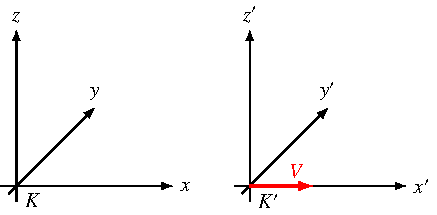
\includegraphics{papers/relativ/tikz/lorentz-trafo-koord.pdf}
    \caption{Bezugssystem \(K\) und ein zweites Koordinatensystem \(K'\),
    welches sich relativ zu \(K\) mit der konstanten Geschwindigkeit \(V\)
    entlang der \(x\)-Achse bewegt.
    \label{relativ:fig:lorentz-trafo-koords}}
\end{figure}
Für den Fall der klassischen Mechanik ist die Transformation einfach und
wir erhalten die Gleichungen
\begin{equation}
    t = t', \quad
    x = x' + Vt, \quad
    y = y', \quad \text{und} \quad
    z = z',
    \label{relativ:eqn:galilei-trafo-beisp}
\end{equation}
sofern man als Startzeitpunkt den Moment wählt,
in dem die beiden Koordinatensysteme am selben Ort sind.
Um den Erhalt des relativistischen Abstands zu gewährleisten,
ergeben sich jedoch (ohne Herleitung) die Gleichungen
\begin{equation}
    t = \frac{t' + \frac{V}{c^2}x'}{\sqrt{1-\frac{V^2}{c^2}}}, \quad
    x = \frac{x' + V t'}{\sqrt{1 - \frac{V^2}{c^2}}}, \quad
    y = y', \quad \text{und} \quad
    z = z'.
    \label{relativ:eqn:lorentz-trafo-beisp}
\end{equation}
